\chapter{BERTrade}

\section{Introduction}
% Context
There is a growing interest in digital humanities for automatic processing and annotation of historical texts. In this work, we study how to take advantage of current NLP models of the BERT family to advance the state of the art in processing historical languages, taking Old French (9th-13th century French) as a use case.

Old French is one of the historical languages for which we have the largest amount of syntactically annotated data and we expect that our results on this example may be generalized and used as a source of inspiration for researchers currently developing annotated resources for other historical languages.

Using contextual word embeddings as input representations has brought clear gains in performances for most of the NLP tasks for which they have been used.
However, this has mostly been attested in languages where sufficient (raw) linguistic data is available.
For less-resourced languages, the most common approach has been to leverage multilingual models such as mBERT \citep{devlin-etal-2019-bert}
%\footnote{The multilingual model is only documented in the supplemental materials at e.g.\ \url{https://github.com/google-research/bert/blob/eedf5716ce/multilingual.md}}

% Motivation
Historical languages are typical cases where available linguistic data is limited, with no chance of acquiring new texts. They are also not normalized by spelling and institutional conventions and tend to be more heterogeneous than contemporary lesser-resourced languages.

Old French is a particularly interesting language for this kind of study, since relatively to its limited amount of available raw text, its volume of \emph{annotated} linguistic data is quite high, due to the existence of the SRCMF dependency treebank \citep{prevost-stein-2013-syntactic} and its latest incarnation in the Universal Dependency project \citep{nivre-etal-2020-universal}, which boasts around \SI{17.7}{K\quantity} sentences\footnote{Putting it in the second place of all French language treebanks in number of sentences.} for around \SI{171}{K\quantity} words.
% The existence of such data is crucial for the evaluation of contextual embeddings, which are essentially tools providing representations for downstream NLP tasks.

Another interesting property of Old French is its proximity to a well-resourced language, namely contemporary French, for which monolingual contextual embeddings models exist and have been shown to be relevant for dependency parsing  \citep{le-etal-2020-flaubert,martin-etal-2020-camembert}.
Last, but certainly not least, the design of an accurate syntactic parser for Old French would be a very valuable tool for computer-assisted linguistic studies.
% Q: Mentionner Profiterole ? Pour justifier la période de nos textes.
% A (LG): Je ne pense pas. Ici on justifie la période par l'utilisation de SRCMF comme probe : on utilise SRCMF donc on reprend la même période.
Indeed, studying the historical variation of syntax in a language that lacks both native speakers and centralized standard variants can be very challenging, due to the prohibitive cost of manual annotations. Automatic syntactic annotations, either as a \enquote{silver-standard} truth or as a bootstrapping step towards manual annotation, can drastically reduce that cost.

In this work, exploiting this currently unique situation of Old French among lesser-resourced and historical languages, we use dependency parsing and POS-tagging of Old French as probes of the relevance of contextual embeddings in a context of high heterogeneity and relative scarcity of data.
More precisely, we consider several neural language models, some of which trained or fine-tuned on a new corpus of raw Old and Middle French texts, and use their internal representations of words as inputs to train taggers and parsers on the SRCMF treebank. The resulting tagging and parsing scores then serve as an evaluation of the quality and usefulness of these representations.
We claim the following contributions:
%
\begin{itemize}
    \item We provide empirical evidence that contextual embeddings are relevant for historical language processing, even when no data is available beyond the treebank used to train a parser.
    \item We provide a comparative study of several strategies for obtaining such contextual embeddings. Specifically we compare cases where raw data is available in the target language and cases where existing contextual embeddings are available for the contemporary counterpart of a historical language.
    \item We release two publicly\footnote{\url{https://url.retained/for/anonymous/review}} available resources for Old French: BERTrade,\footnote{\emph{Bertrade de Laon}, also known as \emph{Berthe au Grand Pied} was the mother of Charlemagne.} a set of contextual word embedding models and a state-of-the art POS-tagging and dependency parsing model.
\end{itemize}

The paper is organized as follows. Section~\ref{sec-related} provides an overview of related work that aims at taking advantage of the BERT family of language models in scenarios where the amount of data is limited. In Section~\ref{sec-data} we provide a description of the dataset we gathered to conduct our experiments and finally we report experiments in Section~\ref{sec-experiments} involving reusing BERT from other languages and training BERT models on Old French.

\section{Related work}
\label{sec-related}
Since the introduction of contextualized word representations \citep{peters-etal-2018-deep,akbik-etal-2018-contextual,devlin-etal-2019-bert} and the many improvements proposed for them in the consumption of computational resources \citep{clark-etal-2020-electra}, in the amount of data required to fine-tune them \citep{raffel-etal-2020-exploring}, and more recently in the length of contextual window \citep{xiong-etal-2021-nystromformer}; there have also been important advancements from a digital humanities point of view on \emph{unsupervised domain adaptation} \citep{ramponi-plank-2020-neural}. In this case one specializes a language model to a particular domain with unlabeled data in order to improve performance in downstream tasks. This can be achieved by  pre-training the models from scratch with specialized data \citep{beltagy-etal-2019-scibert} or by continuing the training of a general model with a new corpus \citep{lee-etal-2019-BioBERT, peng-etal-2019-transfer}. This last method has already been successfully implemented in the context of historical languages, in particular \citet{han-eisenstein-2019-unsupervised} showed that one can successfully adapt the original BERT \citep{devlin-etal-2019-bert} to Early Modern English by continuing the pre-training on historical raw texts.

In a multilingual context, transformer based models such as mBERT have been adapted to low-resource languages and evaluated in dependency parsing and POS-tagging showing promising results \citep{chau-etal-2020-parsing, muller-etal-2021-unseen, gururangan-etal-2020-dont, wang-etal-2020-extending}. However, this multilingual approach has also been criticized for favoring monolingual pre-training even when data is scarce \citep{virtanen-etal-2019-multilingual, ortiz-suarez-etal-2020-monolingual}. Indeed, even when only small pre-training corpora are available, BERT-like models have also been successfully pre-trained resulting in well-performing models \citep{micheli-etal-2020-importance}. Furthermore compact BERT-like models have also been studied \citep{turc-etal-2019-well} and might prove useful in data constrained conditions such as monolingual pre-training of contextualized word representation for low-resource languages.

%BERT for parsing low-resource languages: \citet{chau-etal-2020-parsing} (post-training mBERT with vocabulary augmentations, contemporary languages), \citet{muller-etal-2021-unseen} (post-training mBERT and from scratch, translitteration/normalization, contemporary languages), \citet{gururangan-etal-2020-dont} ("domain adaptative" pre-training).

% Bougé de la section expérience:
% > Many aspects of training contextual word embedding models on very limited amounts of data are still unclear. \citet{micheli-etal-2020-importance} shows that training a small BERT model (by limiting its depth) can yield a valuable model even with as little as \SI{100}{\mebi\byte} of data.
% > However, their objective was more to train a \emph{small} model than an \emph{optimal} one.
% > It is also the approach used by \citet{muller-etal-2021-unseen} for training BERT models on lesser-resourced languages.

Regarding corpora for historical languages, very few of them have manually annotated syntactical resources for their medieval states. English has three such treebanks \citep{oxford-2001-the,kroch-etal-2000-the,traugott-pintzuk-2008-coding} for Old and Middle English. The TOROT treebank for Old Church Slavonic, Old East Slavonic and Middle Russian is another large resource \citep{berdicevskis-eckhoff-2020-diachronic}. To our knowledge, the last large treebank containing medieval texts is IcePaHC for Icelandic \citep{rognvaldsson-etal-2012-icelandic}. Some other corpora were annotated automatically in order to reduce the cost of annotation. For example, \citet{rocio-etal-2003-automated} adapted a parsing pipeline for contemporary Portuguese and \citet{lee-kong-2014-a} used a previously annotated treebank \citep{lee-kong-2012-dependency} to parse a larger medieval Chinese corpus. Concerning contemporary regional Romance languages, \citet{miletic-etal-2020-building} also used a smaller treebank to generate new annotations, and concluded that using similar languages to train a model does not improve parsing. Although there are many resources for Latin, and some for Ancient Greek, we do not include them here, because they do not face the same challenges as medieval states of language, in particular the high level of spelling variability.

Lastly, concerning dependency parsing and POS-tagging of Old French in particular, the works of \citet{guibon-etal-2014-parsing} and \citet{stein-2014-parsing, stein-2016-old} are noteworthy. However they use very different approaches to the one used in this paper and evaluate on previous versions of SRCMF, with incompatible annotation choices and slightly different texts. For the UD version of SRCMF, the most notable work is that of the winner of the \emph{CoNLL 2018 Shared Task} \citep{zeman-etal-2018-conll}, UDPipe 2.0 \citep{straka-2018-udpipe}, which was later enhanced by including contextualized word embeddings \citep{straka-strakova-2019-evaluating}.

% Q: Ajouter POS-tagging and lemmatization using joint learning \citep{pie2019ImprovingLemmatizationNonStandard}.
% A (LG): Pas les mêmes techniques que nous, pas tout à fait le même dataset et les résultats sont pas très simples à extraire du papier, je propose qu'on s'en passe.
% (MR) A : d'accord !

\section{Data}\label{sec-data}

\begin{figure}[thb]
    \centering
    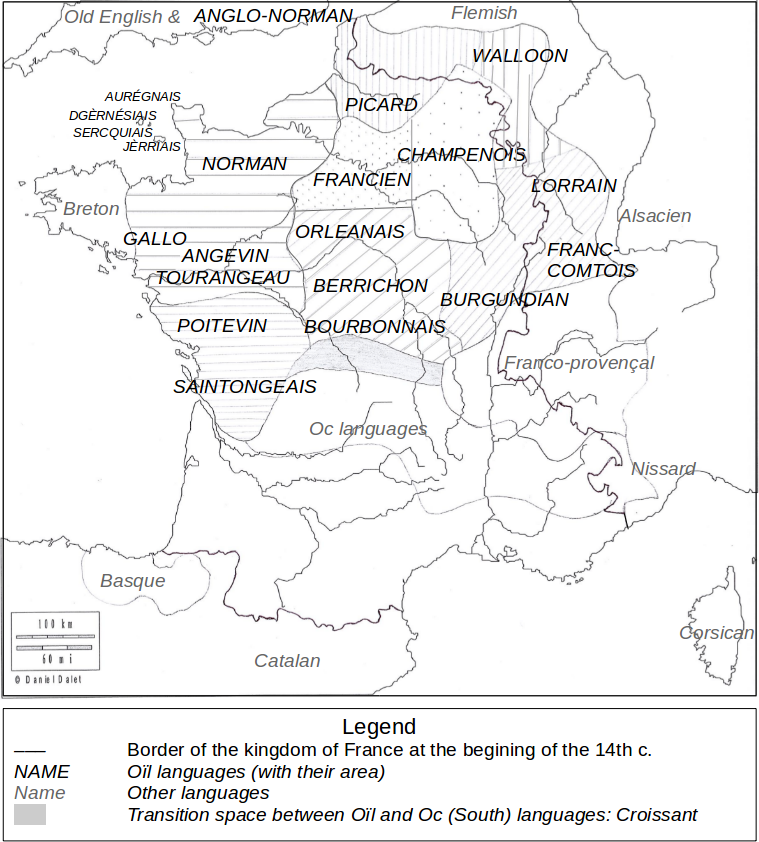
\includegraphics[scale=0.29]{static/media/models/bertrade/map-dialects2.png}
    \caption{Oïl languages}
    \label{fig:map-dialects}
\end{figure}

This section describes the raw corpus of Medieval French we gathered in order to train unsupervised language models for Old French.
To our knowledge, it is one of the largest such dataset gathered for Medieval French, it remains quite small (\SI{55}{\mebi\byte} in total) relatively to the corpora usually used for pre-training contextual embeddings models.

Medieval French covers both Old French (9th-13th c.) and Middle French (14th-15th c.). These stages are linguistically close and both precede the adoption of spelling norms. Middle French is more regular than Old French in some respects such as word order \citep{marchello-Nizia-etal-2020-grande} and less in others such as NP structure and pronouns system \citep{marchello-nizia-etal-1979-histoire}. Medieval French covers a set of \textit{Oïl} Romance languages spoken in the kingdom of France between the 9th and the 15th century (\cref{fig:map-dialects}).
There are around twenty such languages.

Older texts are close to Late Latin, and verse is prevalent until the end of the 13th century. Old French has a relatively free word order.
Until the mid-11th century, the prevalent order is \textit{Subject-Object-Verb} (SOV), which is then gradually supplanted by SVO, which is the default order in contemporary French.
%Unlike most languages with free word order, word functions are not usually given by morphological clues, such as the rich case system of Classical Latin and there are many cases of syntactic ambiguity.
Unlike most languages with free word order, the functions of verbal arguments are not always given away by morphological clues, the already simplistic %\footnote{As compared to that of Latin, for instance.} 
case system of Old French disappears progressively through the covered period.

There are also many cases of syntactic ambiguity. For example, in the following quote from \emph{Lancelot},\footnote{In the edition from Pierre Kunstmann, from the online \textit{Base de français médiéval}: \url{http://catalog.bfm-corpus.org/CharretteKu}.} (verse ~5436),
both \enquote{la dame} and \enquote{Lancelot} could be the subject or the object of \enquote{Vit} and only the context enables the reader to understand that \enquote{la dame} is the subject.

\digloss{Dolant et pansif Lancelot Vit la dame}
{Mournful and meditative Lancelot saw the lady}
{The lady saw that Lancelot was mournful and meditative.}

Word order is also relatively free within constituents. For example, a noun modifier can be on the left or on the right of its governor, and it is not necessarily preceded by a preposition. In contemporary French, it can only appear on the right, and it is found without a preposition only in some cases like named entities. Because of the general free word order and the absence of punctuation in our treebank, this adds up to the ambiguity of the analysis.

In each of the following examples from the SRCMF corpus, the noun following \emph{roi} (\enquote{king}) has a different analysis: head of \emph{roi}, modifier, argument of the same verb or a different one, with no explicit marking:

\begin{center}
    % beroul. modifieur à gauche.
    \begin{dependency}[theme=simple]
        \begin{deptext}[row 2/.style={font=\small}]
            \textit{Fus} \& \textit{tu} \& \textit{donc} \& \textit{pus} \& \textit{a} \& \textit{la} \& \textbf{\textit{roi}} \& \textit{cort} \\
            %VERB \& PRON \& ADV \& ADV \& ADP \& DET \& NOUN \& NOUN \\
            Were \& you \& then \& no more \& at \& the \& king \& court \\
        \end{deptext}
        \depedge{8}{7}{nmod}
        \depedge[edge start x offset=0.5em]{8}{6}{det}
        \depedge[edge start x offset=1em]{8}{5}{case}
    \end{dependency}

    \raggedright
    \enquote{Then were you not at the king's court anymore?} (\emph{Beroul Tristan})
\end{center}

\begin{center}
    % Graal. modifieur à droite.
    \begin{dependency}[theme=simple]
        \begin{deptext}[row 2/.style={font=\small}]
            \textit{la} \& \textit{fille} \& \textit{au} \& \textit{riche} \& \textbf{\textit{roi}} \& \textit{pescheor} \\
            the \& daughter \& of the \& rich \& king \& fisher \\
        \end{deptext}
        \depedge{5}{6}{flat}
    \end{dependency}

    \raggedright
    \enquote{the daughter of the rich Fisher King} (\emph{Queste del Saint Graal})
\end{center}

\begin{center}
    % Roland. arguments du même verbe.
    \begin{dependency}[theme=simple]
        \begin{deptext}[row 2/.style={font=\small}]
            \textit{De} \& \textit{Guenelun} \& \textit{atent} \& \textit{li} \& \textbf{\textit{reis}} \& \textit{nuveles} \\
            From \& Ganelon \& waits \& the \& king \& news \\
        \end{deptext}
        \depedge{3}{5}{nsubj}
        \depedge[edge start x offset=-0.5em]{3}{6}{obj}
    \end{dependency}

    \raggedright
    \enquote{The king waits for news from Ganelon.} (\emph{Chanson de Roland})
\end{center}

\begin{center}
    % Graal. arguments de verbes différents, et absence de ponctuation.
    \begin{dependency}[theme=simple]
        \begin{deptext}[row 2/.style={font=\small}]
            \textit{Biax} \& \textit{sire} \& \textit{fet} \& \textit{li} \& \textbf{\textit{rois}} \& \textit{escu} \& \textit{vos} \& \textit{envoiera} \& \textit{Diex} \\
            Dear \& Sir \& says \& the \& king \& shield \& you \& send-FUT \& God \\
        \end{deptext}
        \depedge{3}{5}{nsubj}
        \depedge{8}{6}{obj}
    \end{dependency}

    \raggedright
    \enquote{Dear Sir, says the king, God will send you a shield.} (\emph{Queste del Saint Graal})
\end{center}

Furthermore, overt subjects are not mandatory, and are often dropped in texts written in verses until the 12th century, after which the presence of subjects increases through time.
These phenomena are particularly prevalent in verse, where metric and rhyming constraints often lead to more contrived syntactic forms than in prose.

Another source of ambiguity is the variety of spellings, due to the lack of spelling standard. For example, the word \textit{moult} (transl. \textit{a lot (of), very}), emblematic of this period, is initially an adjective, and it is progressively grammaticalized, becoming an adverb. Several forms appear at the same time, some with a declension, some without, and the radical does not have a fixed spelling: \textit{molt(e)(s), molz, mult(e)(s), mul(t)z, mou(l)t}…

We chose to include a few texts from the early Middle French period (14th-15th c.) in this raw corpus, which brings a valuable complement of the prose documents that are lacking for Old French, while staying close enough to late Old French, the boundary between the two epochs being somewhat fuzzy.
These texts precede the adoption of norms established by editors using Gutenberg's printing press. Middle French is more regular than Old French in some respects such as word order \citep{marchello-Nizia-etal-2020-grande} and less in others such as NP structure and pronouns system \citep{marchello-nizia-etal-1979-histoire}, but they share most of their lexicon and for these relatively early texts, the syntax is not too different from that of late Old French texts.

%Corpora
\begin{table}[thb]
    \centering
    \tablefontsize
    \begin{tabular}{l S[table-format=2.1]}
        \toprule
        {\textbf{Corpus}}                                  & {\textbf{Size / \si{\mebi\byte}}} \\ %& {\textbf{\# texts}}
        \midrule
        BFM \citep{guillot-etal-2018-base}                & 20.7                              \\ %139
        AND \citep{rothwell-etal-2005-anglo}           & 17.2                              \\ %73
        NCA \citep{kunstmann-stein-2007-le}                       & 9.7                               \\ %271
        Chartes Douai \citep{glessen-2003-elaboration}     & 3.1                               \\ %1
        OpenMedFr \citep{wrisley-2018-the}                 & 1.7                               \\ %19
        Geste \citep{camps-etal-2019-geste}                 & 1.5                               \\ %32
        MCVF \citep{martineau-2008-un}        & 1.4                               \\ %17
        Chartes Aube \citep{reenen-etal-2007-chartes} & 0.2                               \\ %75
        \midrule
        Total                                              & 55.3                              \\ %627
        \bottomrule
    \end{tabular}
    \caption{Data collection}
    \label{tab:texts_train}
\end{table}

\begin{figure}[thb]
    \centering
    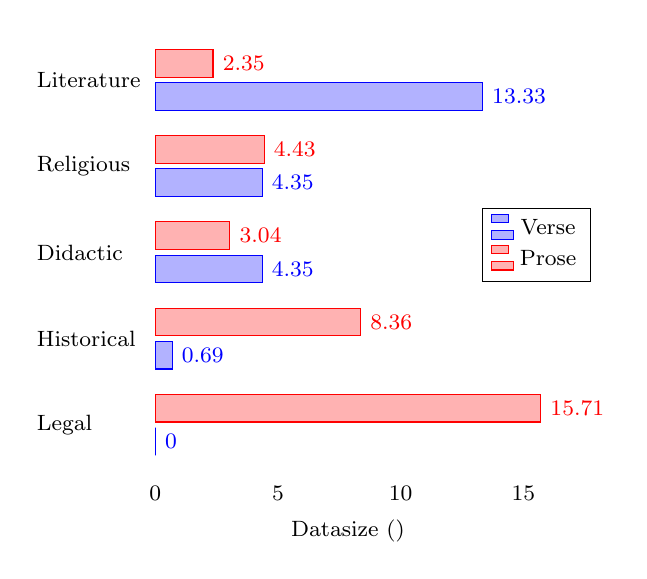
\begin{tikzpicture}
        \begin{axis}[
                xbar,
                font=\footnotesize,
                yticklabel style={text width=0.4cm, align=right},
                y axis line style = { opacity = 0 },
                xlabel = Datasize (\si{\mebi\byte}),
                %axis x line       = none,
                tickwidth         = 0pt,
                ytick             = data,
                %enlargelimits=0.15,
                enlarge y limits  = 0.15,
                enlarge x limits  = 0.2,
                symbolic y coords = {Legal, Historical, Didactic, Religious, Literature},
                nodes near coords,
                legend style={at={(0.95,0.6)}},
            ]
            \addplot
            coordinates {(13.3321,Literature) (4.35204,Religious)
                    (4.35204,Didactic) (0.687576,Historical) (0,Legal)};
            \addplot
            coordinates {(2.352817,Literature) (4.433186,Religious)
                    (3.041925,Didactic) (8.362256,Historical) (15.705591,Legal)};
            \legend{Verse,Prose}
        \end{axis}
    \end{tikzpicture}
    \caption{Distribution of form and domain, gathered from documents metadata and manual annotation.}
    \label{fig:metadata}
\end{figure}

Medieval French has many factors of variation: language evolution, dialects, domains, forms and lack of standard. Our dataset gives us a representation of Medieval French (9th-15th c.) that is as accurate and diversified as possible, given the limited amount of material that survived to these days. The detailed instructions to replicate this dataset are described in the Appendix. No particular processing is done on the original documents.

In order to get a sound evaluation of the contextual embeddings trained with this dataset, we filter out the documents that are also present in the SRCMF treebank used for evaluation purposes in section \ref{sec-experiments}\footnote{As noted by \citet{gururangan-etal-2020-dont}, pre-training on task specific data provides an additional boost, that would muddle our results, since our objective here is not so much task optimization as embeddings benchmarking.}.
The resulting corpus is quite heterogeneous: legal texts and verse literature are in majority, whereas other domains, such as historical and didactic texts, are under-represented, as can be seen in \cref{fig:metadata}.

\section{Experiments}
\label{sec-experiments}
We evaluate a set of alternative word representations on Old French, using their usefulness for POS-tagging and dependency parsing as a downstream evaluation.
To that end, we use the annotated treebank of Old French (SRCMF,  \citet{prevost-stein-2013-syntactic}) as provided by the 2.7 version of the UD dataset \citep{zeman-etal-2020-universal} as a reference treebank.

Our parser/tagger probe uses \citet{dozat-manning-2018-simpler}'s neural graph parser made as reimplemented by \citet{le-etal-2020-flaubert} and \citet{grobol-crabbe-2021-analyse}, using the same hyperparameters.
Word representations are obtained by concatenating subword embeddings, averaged over transformer layers together with character embeddings and non contextualized word embeddings.  %without weighting or scaling. 
%returned by the various models with character embeddings and word embeddings learned together with the parsing model on the treebank train set.
This representation is similar to those used by \citet{straka-strakova-2019-evaluating,ling-etal-2015-finding}.
In all of our experiments, the contextual embeddings are fine-tuned while training the parser.
%\footnote{For a more comprehensive review of the hyperparameters, see the appendix.}.
Unlike the recent CoNLL challenges settings, we assume gold tokenization, since the syntactic annotations we target provide a reference word-based segmentation. Using a predicted one could only add noise to our experiments.
Furthermore for most European languages using a Latin script---including Old and Middle French---, word segmentation is acceptably approximated by simple typographic tokenization.

The remaining of this section presents our experimental results, sorted by nature of required data.
We report UPOS POS-tagging scores as well as unlabeled and labeled attachement scores for dependency parsing (respectively UAS and LAS), as given by the CoNLL-2018 scorer, computed on the development set of SRCMF to avoid overfitting the architecture and transfer learning procedure to the test set.
Results on the test set are provided only for the dev-best models to allow us to compare our results to the state of the art.

Due to the number of costly experiments,\footnote{See the Appendix for elements on the carbon footprint of our experiments.} the results are reported on single runs.
The results should therefore be interpreted  only with respects to the broad trends: small score differences between competing settings should be taken with care.

\subsection{Baselines}\label{sec|baselines}
\begin{table}[thb]
    \centering
    \tablefontsize
    \begin{tabular}{l*{3}{S[table-format=2.2]}}
        \toprule
        {\textbf{Embeddings}} & {\textbf{UPOS}} & {\textbf{UAS}} & {\textbf{LAS}} \\
        \midrule
        Vanilla               & 93.51           & 87.60          & 81.54          \\
        Random-base           & 93.17           & 86.97          & 80.71          \\
        finBERT               & 94.44           & 88.44          & 82.47          \\
        \bottomrule
    \end{tabular}
    \caption{Results on SRCMF dev — no additional data.}\label{tab|nodata}
\end{table}

We first compare a baseline where contextual embeddings are not used at all (Vanilla) with two settings using models with no preexisting knowledge of Old French: Random-base, a randomly initialized model using the same architecture and model size as RoBERTa-base \citep{liu-etal-2019-roberta} %and CamemBERT-base \citep{martin-etal-2020-camembert}, 
and finBERT \citep{virtanen-etal-2019-multilingual}, a contextual embedding model from Finnish, an Uralic language that is unrelated to Old French.
These baselines are meant to check that the gain in performances observed when using models with some (possibly indirect) knowledge of Old French are linked to this knowledge and not simply due to an increase in the number of trainable parameters (for the random baseline) or to a weight distribution induced by training on a language modeling task that would be universally good for all languages (for the finBERT baseline, which can thus be seen as a different kind of weight initialization).

\Cref{tab|nodata} shows the results obtained in these configurations, which show that using a model with random weights, even fine-tuned for these tasks, does not bring any improvement, and is in fact even worse than using no contextual embeddings at all.
In contrast, using a model that has been pretrained for language modeling---even for an unrelated language---brings some modest improvements.
This suggests that pretraining gives a structure to this kind of model that makes it suitable for fine-tuning on the downstream task, but the impact of this gain is clearly---and predictably---very limited compared to what can be expected for representations that have been trained on relevant linguistic data.

\subsection{With related contextual embeddings}\label{sec|related}

\begin{table}[thb]
    \centering
    \tablefontsize
    \begin{tabular}{l*{3}{S[table-format=2.2]}}
        \toprule
        {\textbf{Base model}} & {\textbf{UPOS}} & {\textbf{UAS}} & {\textbf{LAS}} \\
        \midrule
        FlauBERT              & 95.70           & 90.43          & 85.45          \\
        CamemBERT             & 95.86           & 91.15          & 86.31          \\
        mBERT                 & 96.06           & 91.52          & 86.83          \\
        \bottomrule
    \end{tabular}
    \caption{Results on SRCMF dev — monolingual models.}\label{tab|pre-trained}
\end{table}

When a low-resource language is close to a well-resourced one, it is possible to leverage models designed for the latter.
For Old French, contemporary French is an obvious candidate and two contextual embeddings models are available: FlauBERT \citep{le-etal-2020-flaubert} and CamemBERT \citep{martin-etal-2020-camembert}.
Furthermore, mBERT \citep{devlin-etal-2019-bert}, a model trained on multilingual corpus which does not include Old French (possibly apart from some fragments in its contemporary French training data), has been shown to be suitable for many languages, and in particular for Indo-European and Romance languages \citep{straka-strakova-2019-evaluating,muller-etal-2021-unseen}.
We report in \cref{tab|pre-trained} the results obtained when using these language models directly, without addition fine-tuning involving Old French data.

As expected, these results show significant improvements over the baselines, confirming that using contextual embeddings for a related language works better than both randomly initialized embeddings and embeddings pretrained for an unrelated language---even after fine-tuning.
More surprisingly, the best results here are obtained with mBERT.
This could mean that mBERT benefits from having been pretrained for a wider range of languages, including in particular other Romance languages that share with Old French some features,% lost in contemporary French---
for instance null subjects.

\subsection{With raw linguistic data}\label{sec|withraw}

\begin{table*}[ht]
    \centering
    \tablefontsize
    \begin{tabular}{
        l@{\hskip 2ex}
        S[table-format=2.0]
        S[table-format=2.0]
        S[table-format=3.0]@{\hskip 2ex}
        *{3}{S[table-format=2.2]}
        }
        \toprule
        {\textbf{Name}} & {\textbf{Layers}} & {\textbf{Embeddings}} & {\textbf{Heads}} & {\textbf{UPOS}} & {\textbf{UAS}} & {\textbf{LAS}} \\
        \midrule
        BERTrade-tiny   & 2                 & 128                   & 2                & 94.03           & 88.66          & 82.79          \\
        % mini    & 4  & 256 & 4  & 92.60 & 86.48 & 80.12\\
        BERTrade-small  & 4                 & 512                   & 8                & 96.53           & 86.30          & 87.49          \\
        BERTrade-petit  & 12                & 256                   & 4                & 97.14           & 91.90          & 89.18          \\
        BERTrade-medium & 8                 & 512                   & 8                & 96.62           & 91.92          & 87.60          \\
        BERTrade-base   & 12                & 768                   & 12               & 96.74           & 92.37          & 88.42          \\
        % \midrule
        % FastText & {-} & {-} & 00.00 & 00.00 & 00.00\\
        \bottomrule
    \end{tabular}
    \caption{Results on SRCMF dev — Performances of different model sizes when training from scratch}\label{tab|fromscratch}
\end{table*}

\begin{table}[tbh]
    \centering
    \tablefontsize
    \begin{tabular}{l*{3}{S[table-format=2.2]}}
        \toprule
        {\textbf{Base model}} & {\textbf{UPOS}} & {\textbf{UAS}} & {\textbf{LAS}} \\
        \midrule
        BERTrade-petit        & 97.14           & 92.95          & 89.18          \\
        \midrule
        BERTrade-finBERT      & 96.28           & 92.12          & 87.92          \\
        BERTrade-mBERT        & 96.95           & 93.33          & 89.60          \\
        BERTrade-CamemBERT    & 97.16           & 93.75          & 90.06          \\
        BERTrade-FlauBERT     & 96.94           & 93.75          & 90.07          \\
        \bottomrule
    \end{tabular}
    \caption{Results on SRCMF dev — using raw data.}\label{tab|post-train}
\end{table}

We now try to take advantage of the raw Medieval French data described in section \ref{sec-data}.
To that end, we explore two strategies: training a model from scratch and refining existing models by \enquote{post-training} them---running a few more training epochs on the Medieval French raw data.

In the \enquote{from scratch} strategy we first train a BBPE sub-word tokenizer \citep{wang-cho-etal-2020-neural}
on our raw corpus, then train a RoBERTa \citep{liu-etal-2019-roberta} masked language model.
Taking inspiration from \citet{micheli-etal-2020-importance}, who worked in a setting close to ours: a small and noisy pre-training corpus used to create a model from scratch, we used a RoBERTa architecture.
%Since there are no clear silver bullets when it comes to Transformer-based contextual embedding models, the RoBERTa architecture is chosen mostly for comparison with 
As reported in table \cref{tab|fromscratch} we tested several parametrizations of the architecture
also inspired by \citet{turc-etal-2019-well}.
Out of these alternatives, the \enquote{BERTrade-petit} configuration was the
most successful and this is the one we keep for the following experiments.

For the \enquote{post-training} strategy, we continue the training of the pre-trained models used in \cref{sec|baselines,sec|related}, for \num{12} epochs on our raw corpus. We used the same RoBERTa masked language modeling task, using the same parameters as \citet{wang-etal-2020-extending} (but without vocabulary modifications), resulting in the BERTrade-X models, where X is the name of the base model.

The results of these experiments are reported in \Cref{tab|post-train}.
Comparing these to our results of \cref{sec|related} shows that training a model from scratch, even on such limited amounts of data, yields a better model than a simple task-specific fine-tuning of mBERT.
However, post-training mBERT yields even better results, and the best ones are obtained by post-training the models for contemporary French.

\begin{table}[thb]
    \centering
    \tablefontsize
    \begin{tabular}{l*{3}{S[table-format=2.2]}}
        \toprule
        {\textbf{Model}}                                     & {\textbf{UPOS}} & {\textbf{UAS}} & {\textbf{LAS}} \\
        \midrule
        \citet{straka-strakova-2019-evaluating} & 96.26           & 91.83          & 86.75          \\
        \midrule
        mBERT                                                & 96.19           & 92.03          & 87.52          \\
        BERTrade-petit                                       & 96.60           & 92.20          & 87.95          \\
        BERTrade-mBERT                                       & 97.11           & 93.86          & 90.37          \\
        BERTrade-FlauBERT                                    & 97.15           & 93.96          & 90.57          \\
        BERTrade-CamemBERT                                   & 97.29           & 94.36          & 90.90          \\
        \bottomrule
    \end{tabular}
    \caption{Results on SRCMF test}\label{tab|sota}
\end{table}

\subsection{Putting it all together}
Finally, in \cref{tab|sota}, we compare the performances of our models on the test set of SRCMF with those obtained by  \citet{straka-strakova-2019-evaluating}, with similar methods. The difference between the models is that we fine tune the word embeddings while
\citet{straka-strakova-2019-evaluating} keep them frozen.

Our mBERT baseline, which is the closest to their configuration, shows that even without any additional data, task-specific fine-tuning already brings significant improvements, while our models refined using our raw corpus of Medieval French bring further improvements, leading to state of the art results that are consistent with their results on the development set.

\section{Conclusion}

In this work, we have shown that building a monolingual contextual word embeddings model for Medieval French is possible even with limited and heterogeneous linguistic data and that it can bring significant performance gains in parsing and POS-tagging.
To that end, the best strategy seems to be post-training a contextual word embedding model for contemporary French on raw Medieval French documents.
We have not directly addressed the internal heterogeneity issue in both our pretraining and fine-tuning data, relying instead on the versatility of the representation models we considered to bypass it, but it seems a promising perspective for future work---for instance by using finer-grained post-training concentrating on specific linguistic sub-periods or genres.

For historical languages in general, this suggests that language-specific fine-tuning is more efficient when applied to a model pre-trained for their contemporary counterpart than when applied to a multilingual model.
While this study is not currently easy to replicate for other languages due to the lack of annotated data for a suitable downstream task, it suggests that the considerable amount of work required to gather even a small amount of raw texts in the target language is a sound investment, given the significant improvements it can bring to contextual word representations.
Beyond historical languages, these findings could also help for processing minority dialectal variants and contact languages of well-resourced languages and we leave for future work the exploration of these generalizations.

\section{Collecting the data}
\label{subsec:collectdata}
%\todo{Complete AND, MCVF, and Chartes Douai}
The following data can be downloaded directly from their website:
\begin{itemize}
    \item Chartes de l'Aube: \\ \url{https://sites.google.com/site/achimstein/research/resources} \\
          Extract raw text from XML files: <body>, then <s>, then <word>.
    \item Geste: \\ \url{https://github.com/Jean-Baptiste-Camps/Geste} \\
          Raw text is available under /txt/norm/.
    \item OpenMedFr: \\ \url{https://github.com/OpenMedFr/texts} \\
          Remove the header of each file (until \textit{*** START}), its last line (\textit{*** END}), paragraph brakes (\textit{\#|}) and folios or pages numbers.
\end{itemize}

Special permissions are required to access and use these sources:
\begin{itemize}
    \item AND: \\ \url{https://anglo-norman.net/project-members}
    \item BFM: \\ \url{http://bfm.ens-lyon.fr/spip.php?article19} \\
          Raw text is available.
    \item Chartes Douai: \\
          \url{https://www.rose.uzh.ch/docling}
    \item MCVF: \url{http://www.voies.uottawa.ca}
    \item NCA: \\ \url{https://sites.google.com/site/achimstein/research/resources} \\
          Extract raw text from the XML files: <body> then <txm:form>.
\end{itemize}

% \subsection{Oïl languages}
% \begin{figure}[h]
%     \centering
%     \includegraphics[scale=0.3]{map-fr.png}
%     \caption{Map of Medieval Languages}
%     \label{fig:my_label}
% \end{figure}

\section{Details on the models}

\subsection{Models trained from scratch}

These are trained for \num{32} epochs in a masked language modeling task using the same parameters as RoBERTa \citep{liu-etal-2019-roberta} but a smaller batch size of \num{256} samples\footnote{Preliminary experiments with larger batch sizes showed no significant improvement to compensate for the heavier computational load.}, which amounts to a magnitude of \num{e5} steps.
We also use a smaller vocabulary size (\num{8192}) than other works, in line with the observations of \citet{ding-etal-2019-call} that learning large vocabularies on small corpora defeats the purpose of sub-word tokenization.
Using a larger vocabulary size of \num{5e4} (like FlauBERT) also did not seem to bring any improvements in our preliminary experiments and made pre-training more expensive.

\subsection{Post-training}

The pretrained models we used in the post-training settings are those available in the 4.2.0 version of Huggingface Transformers \citep{wolf-etal-2020-transformers} and the exact handles are:

\begin{description}
    \item[mBERT] \href{https://huggingface.co/bert-base-multilingual-cased}{bert-base-multilingual-cased}
    \item[flauBERT] \href{https://huggingface.co/flaubert/flaubert_base_cased}{flaubert/flaubert\_base\_cased}
    \item[camemBERT] \href{https://huggingface.co/camembert-base}{camembert-base}
    \item[finBERT] \href{https://huggingface.co/TurkuNLP/bert-base-finnish-cased-v1}{TurkuNLP/bert-base-finnish-cased-v1}
\end{description}

The post-trained models are those with MLM heads, which we did not reset before post-training, so the post-training phase can be seen as a language transfer task for masked language modeling out of which we extract a contextual word embeddings model.

\section{Carbon Footprint}\label{carbon-footprint}

\begin{table}[t]
    \centering\small
    \scalebox{0.89}{
        \begin{tabular}{@{}lrrrrr@{}}\toprule
            \textbf{Model}                         & \textbf{Power} & \textbf{\# Models} & \textbf{Hours} & \textbf{kWh$\cdotp$PUE} & \textbf{CO\textsubscript{2}e} \\
            \midrule
            Pre-train                              & 10756          & 11                 & 6              & 11216.36                & 358.92                        \\
            Post-train                             & 1520           & 4                  & 20             & 192.13                  & 6.15                          \\
            \midrule
            \multicolumn{2}{@{}l}{Total emissions} &                &                    &                & 365.07                                                  \\
            \bottomrule
        \end{tabular}
    }
    \caption{Average power draw (Watts), number of models trained, training times in hours, mean power consumption (kWh) and CO\textsubscript{2} emissions (kg); for each setting.}
    \label{tab:carbon-bertrade}
\end{table}

In light of recent concerns about the power consumption and carbon footprint of deep learning models \citep{schwartz-etal-2020-green, bender-etal-2021-on} we report the power consumption and carbon footprint of our main experiments following the approach of \citet{strubell-etal-2019-energy}. Two different configurations were used in our experiments, one for pre-training models from scratch (Pre-train) and another one for continuing the training of existing models (Post-train).

\paragraph{Pre-train:} We use a cluster of 4 machines each one having 8 GPU Nvidia Tesla V100 SXM2 32 Go, 384 of RAM, and two Intel Xeon Gold 6226 processors. One Nvidia Tesla V100 card is rated at around 300 W,\footnote{\href{https://www.nvidia.com/en-us/data-center/v100/}{ Nvidia Tesla V100 specification}} while the Xeon Gold 6226 processor is rated at 125 W,\footnote{\href{https://ark.intel.com/content/www/us/en/ark/products/193957/intel-xeon-gold-6226-processor-19-25m-cache-2-70-ghz.html}{Intel Xeon Gold 6226 specification}}. For the DRAM we can use the work of \citet{desrochers-etal-2016-a} to estimate the total power draw of 384GB of RAM at around 39W. The total power draw of this setting adds up to around 10756 W. We train 11 different models in this configuration.

\paragraph{Post-train:} We use a single machine having 4 GPU Nvidia Tesla V100 SXM2 32 Go, 192 of RAM and two Intel Xeon Gold 6248 processors. The Xeon Gold 6248 processor is rated at 150 W,\footnote{\href{https://ark.intel.com/content/www/us/en/ark/products/192446/intel-xeon-gold-6248-processor-27-5m-cache-2-50-ghz.html}{Intel Xeon Gold 6248 specification}}, and the DRAM total power draw can be estimated at around 20W. The total power draw of this setting adds up to around 1520 W. We train 4 different models in this configuration.

Having this information, we can now use the formula proposed by \citet{strubell-etal-2019-energy} in order to compute the total power required to pre-train one model from scratch:
\[
    p_t = \frac{1.58t(cp_{c} + p_r + gp_g)}{1000}
\]
Where $c$ and $g$ are the number of CPUs and GPUs respectively, $p_c$ is the average power draw (in Watts) from all CPU sockets, $p_r$ the average power draw from all DRAM sockets, and $p_g$ the average power draw of a single GPU. We estimate the total power consumption by adding GPU, CPU and DRAM consumption, and then multiplying by the \emph{Power Usage Effectiveness} (PUE), which accounts for the additional energy required to support the compute infrastructure. We use a PUE coefficient of 1.58, the 2018 global average for data centers \citep{strubell-etal-2019-energy}. In table \ref{tab:carbon-bertrade} we report the training times in hours, as well as the total power draw (in Watts) of the system used to train the models. We use this information to compute the total power consumption of each setting, also reported in table \ref{tab:carbon-bertrade}.

We can further estimate the CO\textsubscript{2} emissions in kilograms of each single model by multiplying the total power consumption by the average CO\textsubscript{2} emissions per kWh in our region which were around 32g/kWh in January 2021,\footnote{Anonymous website reporting average local emission per kWh in January 2021.} when the models were trained. Thus the total CO\textsubscript{2} emissions in kg for one single model can be computed as:
\[
    \text{CO}_{2}\text{e} = 0.032 p_t
\]
All emissions are also reported in table \ref{tab:carbon-bertrade}.
